\documentclass[dvips,12pt]{article}

% Any percent sign marks a comment to the end of the line

% Every latex document starts with a documentclass declaration like this
% The option dvips allows for graphics, 12pt is the font size, and article
%   is the style

\usepackage[pdftex]{graphicx}
\usepackage{url}
\usepackage{amsfonts}
\usepackage{amsmath}
\usepackage{amssymb}
\usepackage[left=3cm,right=2cm,top=2.5cm,bottom=2cm]{geometry}
\newcommand{\R}{\mathbb{R}}
\newcommand{\argmax}[1]{\underset{#1}{\operatorname{arg}\,\operatorname{max}}\;}

% These are additional packages for "pdflatex", graphics, and to include
% hyperlinks inside a document.



% These force using more of the margins that is the default style

\begin{document}

% Everything after this becomes content
% Replace the text between curly brackets with your own

\title{Modelling real world networks using Kronecker graphs}
\author{Gautam Rayaprolu}
\date{\today}

% You can leave out "date" and it will be added automatically for today
% You can change the "\today" date to any text you like


\maketitle

\begin{abstract}
Graphs are a general purpose representation of data which capture relationships (edges) between individual units (nodes). They can be used to model domains ranging from social and computer networks to biological protein protein interactions. In this paper I describe the general properties of real world networks and look at techniques to model these networks. In particular I describe the algorithm outlined in \cite{ghahramani2010} which uses kronecker matrices to model graphs and represent them succinctly. I also present the results of implementing this algorithm and using it to model social network data obtained from \cite{SNAP-dataset}.
\end{abstract}


% This command causes the title to be created in the document

\section{Introduction}
Formally, a graph $G = (V,E)$ is simply a collection of vertices $V$ (nodes) and edges $E$. The edges are simply a set of pairs of vertices which represent a 'link'. Graphs can be undirected or directed depending on whether a edge is 'two-way' or 'one-way'. Different social networks can be thought of as undirected or directed depending on the rules of the website. For example, a network of friends on Facebook would constitute an undirected graph but a graph of 'followers' and 'following' on Instagram is directed because that is not a symmetric relationship. In this paper I will mostly restrict my attention to undirected graphs.

Our problem statement will then be as follows. We will be given a graph $G$ and we wish to be able to summarize its structure succinctly and be able to efficiently generate larger graphs that preserve the properties of the original graph. In order to do this we first need to more formally describe what the 'structure' of the graph means. \cite{watts1998} coined the term 'small-world' networks for social graphs. It describes real world graphs as being highly clustered , having a low diameter and exhibiting a power law degree distribution. The degree of a node is defined as the number of edges leaving the node. The clustering coefficient of a singe node is defined as follows : $$c_u := \frac{2T(u)}{deg(u)(deg(u)-1)}$$ $T(u)$ is the number of triangles that the node $u$ is part of and $deg(u)$ is the degree of the node. The average clustering coefficient of the graph is simply the average value across all nodes. The diameter is defined as the longest 'shortest' path between any 2 nodes on the graph. These will be our main measures of the structure of the graph



\section{Networks and Random Graphs}


\begin{figure}[!htb]
\centering
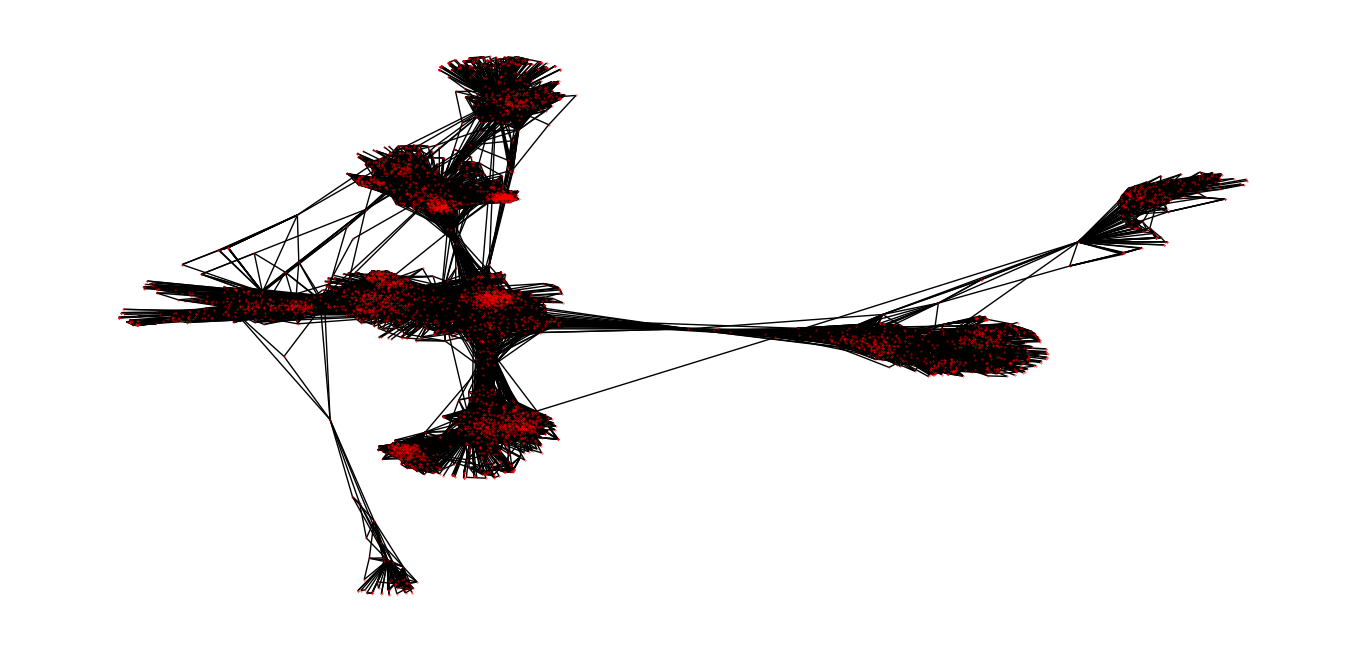
\includegraphics[scale=0.4]{facebook_connectivity_graph}
\caption{Anonymized Facebook friend network}
\label{facebook}
\end{figure}

Figure \ref{facebook} was generated from anonymized facebook friend data obtained from \cite{SNAP-dataset}. In this visualization the 'small-world' properties described in the above section are clearly visible. The average clustering coefficient of this dataset was calculated to be around $0.61$. 

Now that we know the problem at hand, we need to consider the model that we wish to fit to our data. In this paper I will look at random graph models where each edge exists with some probability. The oldest and best known model of random graphs is the erdos-renyi model. The erdos-renyi random graph model $G(n,p)$ is a graph where each of the $n \choose 2$ edges exist with equal probability $p$. This model has a rich mathematical theory behind it but it is a poor model of real world networks (which it wasn't designed for)

\begin{figure}[!htb]
\centering
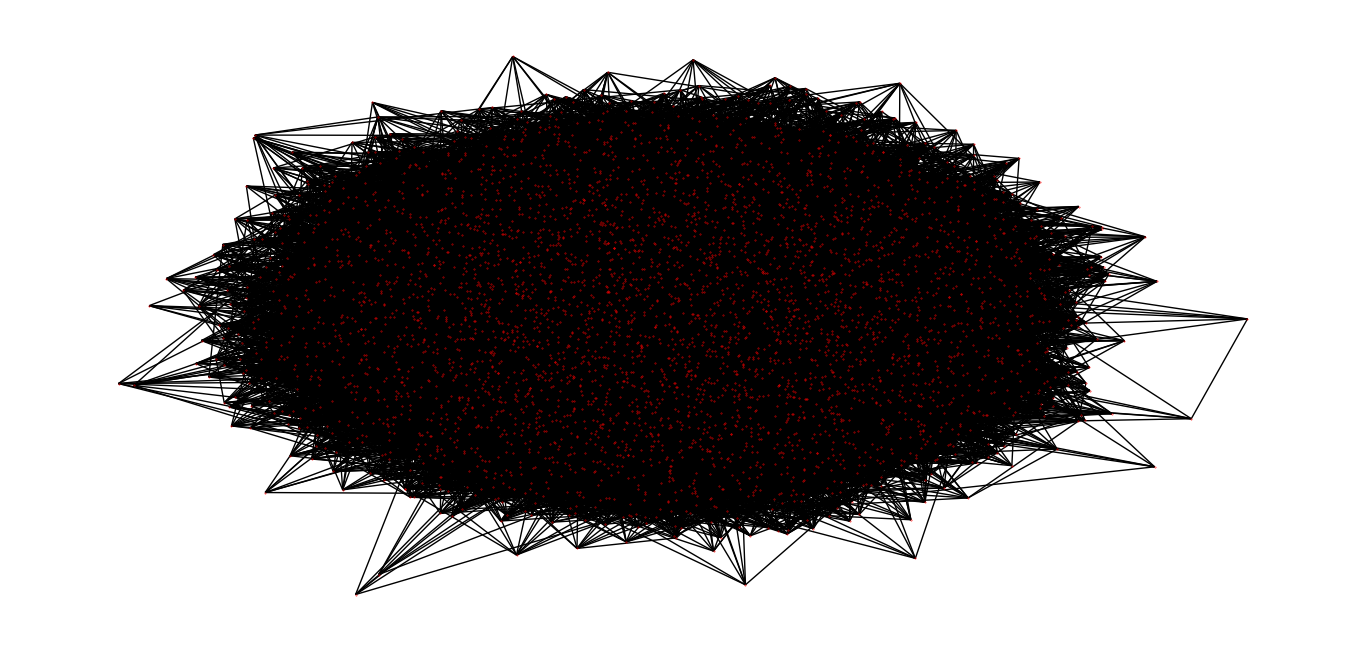
\includegraphics[scale=0.3]{Gnp_connectivity_graph}
\caption{Sample of Erdos-Renyi Graph - $G(4032,0.005)$}
\label{gnp}
\end{figure}

Figure \ref{gnp} was generated on the same number of nodes using a $p$ value such that the expected number of edges is the same as that in Figure \ref{facebook}. Note that this is the maximum likelihood estimate of the parameter. Observe that this leads to a graph topology which is very different from the original dataset. This is because of the inherent nature of the Erdos - Renyi model. It leads to a uniform graph without clustering. The clustering coefficient of the sampled graph in Figure \ref{gnp} is about $0.01$ which is an order of magnitude lower than the facebook graph.

\begin{figure}[!htb]
\centering
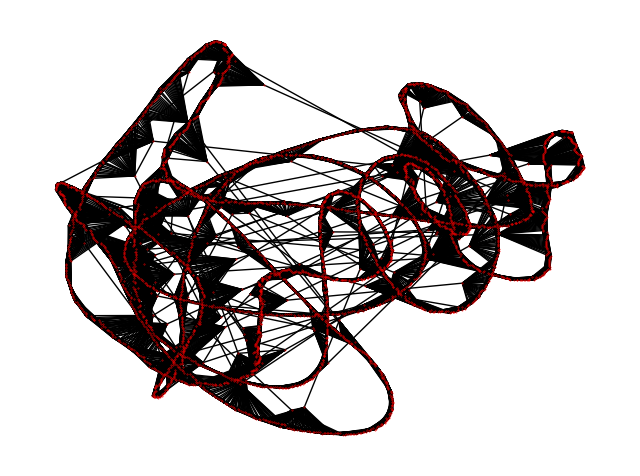
\includegraphics[scale=0.5]{watts_strogatz_connectivity_graph}
\caption{Sample of Watts Strogatz Small World graph}
\label{wssg}
\end{figure}

Another model of random graph generation was proposed by \cite{watts1998}. This model was specifically designed to generate graphs that had the 'small-world' properties that we discussed and is appropriately named the 'watts-strogatz small world graph'. Figure \ref{wssg} is a simulation using this model. Observe that we start to see the clustering behaviour that is characteristic of Figure \ref{facebook}. The average clustering coefficient of this graph is $0.71$ which is actually higher than that of the observed data. This graph is obtained by starting with a ring lattice and replacing edges with a probability $\beta$.  The topology of this graph is determined by this parameter $\beta$. However, due to the nature of the construction there is no easy (computationally efficient) way to learn $\beta$ from training data. 

\section{Kronecker Graphs}

In order to learn graph structure from data \cite{ghahramani2010} suggests the use of Kronecker Graphs. In order to define Kronecker Graphs we first need to define Kronecker multiplication and Kronecker Matrices. Kronecker Multiplication is a matrix operation defined as follows. 
\[
C = A \otimes B = 
\begin{bmatrix}
    a_{11}B       & a_{12}B & a_{13}B & \dots & a_{1n}B \\
    a_{21}B     & a_{22}B & a_{23}B & \dots & a_{2n}B \\
    \hdotsfor{5} \\
    a_{d1}B       & x_{d2}B & a_{d3}B & \dots & a_{dn}B
\end{bmatrix}
\]

Note that if $A$ is $n \times d$ matrix and $B$ is $n' \times d'$ matrix then C is of dimension $n.n' \times d.d'$. In order to generate a Kronecker Graph, we take an initiator adjacency matrix $P$ (generally a small square matrix) and then repeatedly apply the Kronecker product on this matrix till we get an appropriately large adjacency matrix.
\begin{gather}
  C^1 = P \\
  C^k = C^{k-1} \otimes P
\end{gather}

Observe that if P is of size $m \times m$ then $C^k$ will be of size $m^k \times m^k$. This adjacency matrix represents our output graph. Alternatively we could consider a stochastic Kronecker Graph, where the values in our Initiator Matrix are real numbers in $(0,1)$ and perform the same operation. Each element in the output matrix is an independent Bernoulli representing the probability of an edge. We simply sample these variables and output an adjacency matrix.

In \cite{ghahramani2010} they show that Kronecker graphs have a power law degree distribution and constant diameter (when the initiator matrix is chosen appropriately) which makes them good candidates to model real world networks. Now the problem reduces to finding an appropriate initiator matrix. In order to do this we will use a maximum (log)likelihood estimator. 
\begin{gather}
\Theta = \argmax{\Theta} \log P(G|\Theta) \\
\log P(G|\Theta) = \log \sum_{\sigma} P(G|\Theta, \sigma) P(\sigma)
\end{gather}

In the above equations $G$ refers to our training graph on $N = N_1^k$ nodes, $\Theta$ refers to the parameters of the initiator matrix of size $N_1$. In order to compute the likelihood, we need to consider all possible labellings of nodes to rows (columns) of our final stochastic Kronecker matrix obtained from $\Theta$. $\sigma$ represents a single labelling permutation. Note that there are $N!$ labelling permutations, which makes an explicit calculation of this sum intractable even for small $N$. Observe that the log likelihood is a non convex function, since any permutation of the parameters results in the same likelihood value.

In order to get around this problem \cite{ghahramani2010} suggests the use of a metropolis sampling algorithm. Observe that :
\begin{gather}
P(\sigma|G, \Theta)  = \frac{P(\sigma, G, \Theta)}{Z} \\
Z = \sum_{\tau} P(\tau, G, \Theta)
\end{gather}
$Z$ is simply a normalizing constant, which then cancels out when we consider the probability ratio of 2 permutations $$T(\sigma, \sigma') = \frac{P(\sigma| G, \Theta)}{P(\sigma'| G, \Theta)}$$ This suggests a very natural algorithm to generate a random permutation. We first start at some initial permutation. We then uniformly pick two integers $1 \leq i,j\leq N$ and then return the new permutation with probability $T(\sigma, \sigma')$. In order to estimate the log-likelihood, we then simply take a fixed number of random permutations and compute an average over the likelihood values.

A naive approach to calculating the likelihood, given a permutation and the stochastic matrix, takes $O(N^2)$ time, since we need to sum over all the elements in the graph's adjacency matrix. \cite{ghahramani2010} suggests a taylor series approximation that reduces this to $O(|E|)$ where $|E|$ is the number of edges in the graph. In the worst case this can also be $O(N^2)$ but it is often $O(N)$ for real world graphs.


\section{Results}
I implemented the likelihood estimation function using metropolis sampling and the taylor series optimization and then used Scipy's optimization library to find the Maximum Likelihood Estimator for initiator matrices of size $2 \times 2$ and $3 \times 3$. Note that this is a constrained optimization problem where the bounds for the values in the initiator matrix are in the range $(0,1)$. The training data was selected from the adjacency matrix of the graph in Figure \ref{facebook}. Note that the size of the training data has to differ for different sizes of the initiator matrix. I used $2048 = 2^{11}$ nodes to train the $2 \times 2$ initiator and $2187 = 3^7$ nodes for the $3 \times 3$ case. 
\\
\begin{figure}[!htb]
\centering
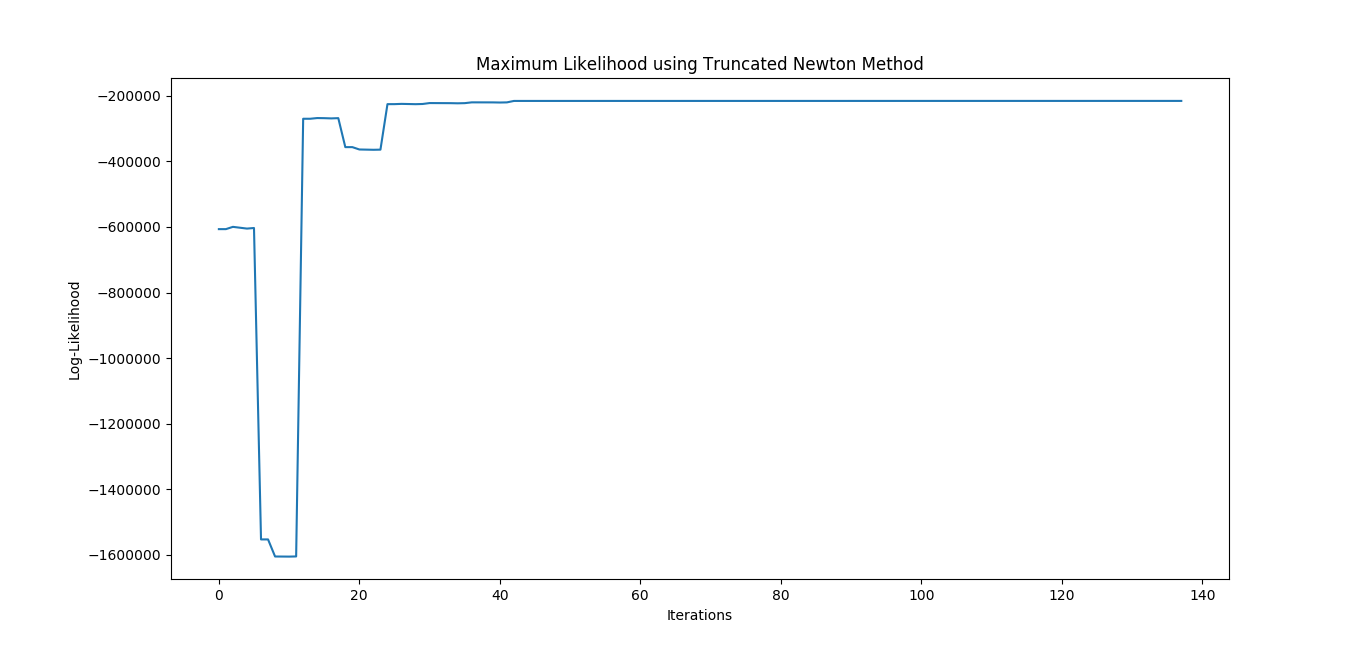
\includegraphics[scale=0.4]{Log-Likelihood-TNC}
\caption{Maximum Likelihood Convergence using Truncated Newton Method}
\label{mlec}
\end{figure}


Scipy's optimization library has multiple methods available for constrained optimization. Note that the function we are minimizing is essentially a log function which is smooth and has derivatives at all points other than $0$. So I decided to use methods that used gradient information. The appropriate methods to test seemed to be 'TNC'(Truncated Newton Method) and the 'L-BFGS-B'. The likelihood estimation function I wrote was fairly computationally intensive, taking upto several seconds for a single function call (the time is not deterministic due to the metropolis sampling). I simply tested the 2 methods on a smaller training set and picked 'TNC' since it seemed to converge faster. Figure \ref{mlec} shows the progression of likelihood values over the course of the optimization. I also used $100$ permutation samples to estimate the sum. This was restricted simply due to time constraints. However, I also tested the likelihood estimate using 1000 and 10000 samples and the estimate remained fairly similar. The $2 \times 2$ initiator matrix obtained from this was 
\[
\begin{bmatrix}
    0.68       & 0.64\\
    0.55     & 0.74
\end{bmatrix}
\]

I then used this initiator matrix to sample a graph of size $8192 = 2^{13}$ which is shown in Figure \ref{kron}. The average clustering coefficient of this graph was calculated to be around 0.008 which makes it a poor model of the original graph. This remained true even when I used a $3 \times 3$ initiator matrix, although the log likelihood values were far better. This is simply a consequence of the fact that a larger initiator matrix has more degrees of freedom so leads to a more expressive model, but one that may be prone to overfitting. In terms of the bias-variance tradeoff, a larger initiator matrix gives us a model with lower bias but higher variance. Since I did not see much of an improvement with a $3 \times 3$ initiator I stuck to the smaller matrix. Training larger initiators was infeasible due to the computational expense involved.

\begin{figure}[!htb]
\centering
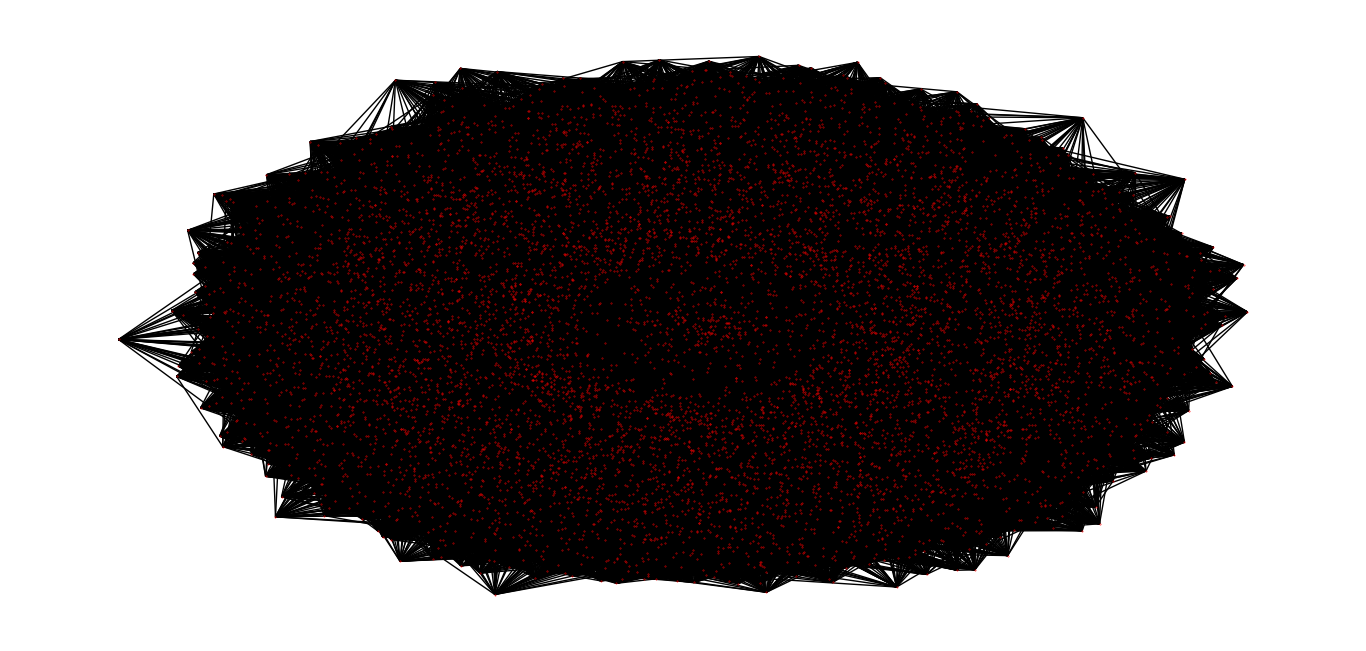
\includegraphics[scale=0.3]{kronecker_graph_P2}
\caption{Learned Kronecker Graph}
\label{kron}
\end{figure}
%write up which one finished faster, show a graph of the log likelihoods


\section{Conclusion}

I started out this project by looking to experiment with techniques to detect specific structures in graphs. The most well known variant of this problem is the planted clique problem, which is described in \cite{cook2015}. On reading the literature I came across \cite{ghahramani2010} which suggested a generative model of graphs using Kronecker matrices to model real world networks. I used social network data from \cite{SNAP-dataset} to train this model using the proposed algorithm. However, the results were not quite as expected. The graph samples from the trained model did not have the distinct features of the social network graph, most notably the clustering property.

There are many possible reasons for this. The optimization problem we are trying to solve is non convex and in \cite{ghahramani2010} they note that there is only a narrow band of parameters where Kronecker Matrices have the interesting properties of real world graphs. This implies that we may need to consider better initial parameter values before running the optimization program. One could also look at larger initiator matrices to see if that made the problem much better. Note that the number of parameters grows as the size of matrix, which makes very large sizes infeasible to test on. It is also possible that the clustering properties of kronecker graphs aren't seen at the relative small scale of $2^{13}$ nodes. However this was the largest sample I could generate using the computing resources available to me. Further work could experiment with any of these to try and get better results.

\newpage

\begin{thebibliography}{99}


\bibitem{berthet2013} 
Berthet Quentin,	
Rigollet Philippe,	
{Computational Lower Bounds for Sparse PCA},(2013).

\bibitem{cook2015} 
Cook Alexis B,	
Miller Benjamin A,
{Planted clique detection below the noise floor using low-rank sparse PCA},(2015).

\bibitem{ghahramani2010}
Jon Kleinberg,
Jure Leskovec,
Deepayan Chakrabarti,
Christos Faloutsos,
Zoubin Ghahramani
{Kronecker Graphs: An Approach to Modelling Networks},(2010).

\bibitem{SNAP-dataset}
Jure Leskovec,
Andrej Krevl
{{SNAP Datasets}: {Stanford} Large Network Dataset Collection}

\bibitem{watts1998}
Duncat Watts,
Steven Strogatz,
{Collective Dynamics of Small World Networks},(1998).




\end{thebibliography}



\end{document}